\documentclass[10pt]{article}\usepackage{graphicx, color}
%% maxwidth is the original width if it is less than linewidth
%% otherwise use linewidth (to make sure the graphics do not exceed the margin)
\makeatletter
\def\maxwidth{ %
  \ifdim\Gin@nat@width>\linewidth
    \linewidth
  \else
    \Gin@nat@width
  \fi
}
\makeatother

\definecolor{fgcolor}{rgb}{0.2, 0.2, 0.2}
\newcommand{\hlnumber}[1]{\textcolor[rgb]{0,0,0}{#1}}%
\newcommand{\hlfunctioncall}[1]{\textcolor[rgb]{0.501960784313725,0,0.329411764705882}{\textbf{#1}}}%
\newcommand{\hlstring}[1]{\textcolor[rgb]{0.6,0.6,1}{#1}}%
\newcommand{\hlkeyword}[1]{\textcolor[rgb]{0,0,0}{\textbf{#1}}}%
\newcommand{\hlargument}[1]{\textcolor[rgb]{0.690196078431373,0.250980392156863,0.0196078431372549}{#1}}%
\newcommand{\hlcomment}[1]{\textcolor[rgb]{0.180392156862745,0.6,0.341176470588235}{#1}}%
\newcommand{\hlroxygencomment}[1]{\textcolor[rgb]{0.43921568627451,0.47843137254902,0.701960784313725}{#1}}%
\newcommand{\hlformalargs}[1]{\textcolor[rgb]{0.690196078431373,0.250980392156863,0.0196078431372549}{#1}}%
\newcommand{\hleqformalargs}[1]{\textcolor[rgb]{0.690196078431373,0.250980392156863,0.0196078431372549}{#1}}%
\newcommand{\hlassignement}[1]{\textcolor[rgb]{0,0,0}{\textbf{#1}}}%
\newcommand{\hlpackage}[1]{\textcolor[rgb]{0.588235294117647,0.709803921568627,0.145098039215686}{#1}}%
\newcommand{\hlslot}[1]{\textit{#1}}%
\newcommand{\hlsymbol}[1]{\textcolor[rgb]{0,0,0}{#1}}%
\newcommand{\hlprompt}[1]{\textcolor[rgb]{0.2,0.2,0.2}{#1}}%

\usepackage{framed}
\makeatletter
\newenvironment{kframe}{%
 \def\at@end@of@kframe{}%
 \ifinner\ifhmode%
  \def\at@end@of@kframe{\end{minipage}}%
  \begin{minipage}{\columnwidth}%
 \fi\fi%
 \def\FrameCommand##1{\hskip\@totalleftmargin \hskip-\fboxsep
 \colorbox{shadecolor}{##1}\hskip-\fboxsep
     % There is no \\@totalrightmargin, so:
     \hskip-\linewidth \hskip-\@totalleftmargin \hskip\columnwidth}%
 \MakeFramed {\advance\hsize-\width
   \@totalleftmargin\z@ \linewidth\hsize
   \@setminipage}}%
 {\par\unskip\endMakeFramed%
 \at@end@of@kframe}
\makeatother

\definecolor{shadecolor}{rgb}{.97, .97, .97}
\definecolor{messagecolor}{rgb}{0, 0, 0}
\definecolor{warningcolor}{rgb}{1, 0, 1}
\definecolor{errorcolor}{rgb}{1, 0, 0}
\newenvironment{knitrout}{}{} % an empty environment to be redefined in TeX

\usepackage{alltt}
\usepackage[english]{babel}
\usepackage{graphicx,color,alltt}
\usepackage{hyperref}
\usepackage{apacite}

\setlength{\parskip}{0.5ex plus0.1ex minus0.1ex}
\setlength{\parindent}{0em}


\hypersetup{%
hyperindex,%
colorlinks,%
linktocpage,%
plainpages=false,%
linkcolor=blue,%
citecolor=blue,%
urlcolor=red,%
pdfstartview=Fit,%
pdfview={XYZ null null null}%
}
\IfFileExists{upquote.sty}{\usepackage{upquote}}{}


\begin{document}

%\SweaveOpts{concordance=TRUE}
%\SweaveOpts{engine=R,eps=FALSE}
%\SweaveOpts{keep.source=TRUE}

%\VignetteIndexEntry{lsttheory: An \textsf{R}  Package for Fast Computation of State Trait Models}
%\VignetteDepends{lsttheory}
%\VignetteKeywords{states, traits, reliability, occasion specificity, consistency}
%\VignettePackage{lsttheory}


\title{\texttt{lsttheory}: An \textsf{R}  Package for Fast Computation of State Trait Models}

\author{
  Axel Mayer\\
  University of Jena
  \and
  Rolf Steyer\\
  University of Jena
  \and
  Christian Geiser\\
  Utah State University
  \and
  David A. Cole\\
  Vanderbilt University
}

\date{\today}
\maketitle

\begin{abstract}
This \textsf{R} \cite{RCoreTeam} package is a supplement for the article 'A Theory of States and Traits' (Steyer, Geiser, Cole, \& Mayer, 2013). It is based on the structural equation modeling \textsf{R} package \texttt{lavaan} (Rosseel, 2012) and provides a convenient interface to compute some common models of the revised latent state-trait theory (LST-R theory). The main function of the package allows for easy specification of multistate, multistate-singletrait, and multistate-multitrait models. It automatically generates \texttt{lavaan} syntax for these models, runs the models, and returns model estimates together with reliability, occasion specificity, and consistency coefficients for the respective models. There is also an additional package called
\texttt{lsttheoryGUI}, which depends on \texttt{lsttheory}. The \texttt{lsttheoryGUI} provides a graphical user interface, i.e., a click menu, for users who are not familiar with \textsf{R}. \texttt{lsttheoryGUI} works best with the JGR console for R (Markus Helbig, Simon Urbanek, \& Ian Fellows, 2013).

\end{abstract}

\noindent
{\bf Keywords:} states, traits, reliability, occasion specificity, consistency \\


\textbf{Cautionary Note:} The package is currently under development and some things may change in the future. We are at an early stage of development and it is likely that the structure and key aspects of the two packages will change. The latest versions can be downloaded from \url{metheval.uni-jena.de}. We also plan to release the package on CRAN, once we are a bit furhter in the develpment process. Please report any bugs.




\newpage
\tableofcontents

\newpage



\section{Introduction} \label{sec:intro}

\texttt{lsttheory} allows for easy specification of multistate, multistate-singletrait, and multistate-multitrait models. This vignette is structured as follows: We first describe the installation process in detail for nonexperienced users of \textsf{R}. Users who are familiar with package installation from local .zip files may wish to skip this section. We then present various kinds of LST-R theory models with syntax and model results.



\section{Installation}

The \textsf{R} package \texttt{lsttheory} will most likely be installed from a local file. Therefore, we need to install the dependencies first. The installation has been tested under Windows 7 and under Linux (Ubuntu 11.10). It should also work under Mac OS X using the JGR console --- but we haven't tested it yet. Please make sure that you are using R version 3.0.1 or higher.

\subsection{Windows Installation}

For a Windows installation (without Rtools) we suggest installing the dependencies from a CRAN mirror first by executing
%
\begin{knitrout}
\definecolor{shadecolor}{rgb}{0.969, 0.969, 0.969}\color{fgcolor}\begin{kframe}
\begin{alltt}
\hlfunctioncall{install.packages}(\hlstring{"lavaan"})  ## for lsttheory
\hlfunctioncall{install.packages}(\hlstring{"Deducer"})  ## for lsttheoryGUI
\end{alltt}
\end{kframe}
\end{knitrout}

%
in the console (either the standard Rconsole or the JGR console) and then selecting a mirror next to you. After that, the \textsf{R} package \texttt{lsttheory} can be installed using the Windows binary file (with file ending .zip) as follows:
%
\begin{knitrout}
\definecolor{shadecolor}{rgb}{0.969, 0.969, 0.969}\color{fgcolor}\begin{kframe}
\begin{alltt}
\hlfunctioncall{install.packages}(\hlstring{"D:/workspace/lsttheory_0.1-1.zip"})
\hlfunctioncall{install.packages}(\hlstring{"D:/workspace/lsttheoryGUI_0.1-1.zip"})
\end{alltt}
\end{kframe}
\end{knitrout}

%
Please adjust the file path and version number accordingly. We recommend using the JGR console (\url{http://rforge.net/JGR/}). The JGR console can be called via a launcher or from with an R session by calling
%
\begin{knitrout}
\definecolor{shadecolor}{rgb}{0.969, 0.969, 0.969}\color{fgcolor}\begin{kframe}
\begin{alltt}
\hlfunctioncall{library}(JGR)
\hlfunctioncall{JGR}()
\end{alltt}
\end{kframe}
\end{knitrout}

%


\subsection{Linux Installation}

We assume that Linux users are familiar with installing \textsf{R} packages from source. The source files are \texttt{lsttheory\_0.1-1.tar.gz} and \texttt{lsttheoryGUI\_0.1-1.tar.gz}. Note that for the graphical user interface to work, the user may want to use the JGR console. The JGR console can be called from with an R session by calling
%
\begin{knitrout}
\definecolor{shadecolor}{rgb}{0.969, 0.969, 0.969}\color{fgcolor}\begin{kframe}
\begin{alltt}
\hlfunctioncall{library}(JGR)
\hlfunctioncall{JGR}()
\end{alltt}
\end{kframe}
\end{knitrout}

%

\subsection{Loading the Package}

After having succesfully installed the packages, we need to load them:
%
\begin{knitrout}
\definecolor{shadecolor}{rgb}{0.969, 0.969, 0.969}\color{fgcolor}\begin{kframe}
\begin{alltt}
\hlfunctioncall{library}(\hlstring{"lsttheory"})
\end{alltt}


{\ttfamily\noindent\itshape\color{messagecolor}{\#\# Loading required package: lavaan}}

{\ttfamily\noindent\itshape\color{messagecolor}{\#\# This is lavaan 0.5-16}}

{\ttfamily\noindent\itshape\color{messagecolor}{\#\# lavaan is BETA software! Please report any bugs.}}\begin{alltt}
\hlcomment{# library('lsttheoryGUI')}
\end{alltt}
\end{kframe}
\end{knitrout}

%
If you are using the JGR console, you can click on default next to the lsttheory and lsttheoryGUI entry in the Package Installer. Then the packages and their dependencies are automatically loaded every time you open JGR.

\newpage
\section{Multistate Models}

The lsttheory pacakge contains several simulated example datasets. The first one that we use is the dataset \texttt{multistate}. It contains 9 manifest variables $Y_{it}$, where the index refers to the $i$th manifest variable assessed at occasion $t$.
%
\begin{knitrout}
\definecolor{shadecolor}{rgb}{0.969, 0.969, 0.969}\color{fgcolor}\begin{kframe}
\begin{alltt}
\hlfunctioncall{data}(multistate)
\hlfunctioncall{head}(\hlfunctioncall{round}(multistate, 2))
\end{alltt}
\begin{verbatim}
##     y11   y21   y31   y12   y22   y32   y13   y23   y33
## 1  3.88  4.76  4.54  3.95  5.68  2.53  2.18  3.74  3.29
## 2  0.02  2.40  2.42  2.52  3.33  0.33  0.08  1.61  0.83
## 3  0.06  1.54 -0.86  0.12 -1.19  1.69  1.59  2.49  0.20
## 4  2.70  3.41  3.31  2.63  1.83  3.29  2.47  2.05  3.34
## 5  0.30  2.03 -0.08  0.46  1.41  1.19 -1.58 -1.40  0.97
## 6 -5.13 -3.78 -3.23 -0.34  1.48 -1.64 -2.36 -3.27 -0.78
\end{verbatim}
\end{kframe}
\end{knitrout}

%

\subsection{Multistate Model with $\eta_t$-Congenericity}

First, we use this dataset to fit a multistate model with $\eta_t$-congenericity and conditional mean independence (see Box 4.1 of SGCM). The main function of our package to be called by the user is \texttt{lsttheory}. See \texttt{?lsttheory} for details. It is used to fit all models. The multistate model with $\eta_t$-congenericity can be specified as follows:


%
\begin{knitrout}
\definecolor{shadecolor}{rgb}{0.969, 0.969, 0.969}\color{fgcolor}\begin{kframe}
\begin{alltt}
m1 <- \hlfunctioncall{lsttheory}(neta = 3, data = multistate)
\hlfunctioncall{print}(m1)
\end{alltt}
\begin{verbatim}
## 
##  Multistate Model 
##  
##     rely spey cony
## y11 0.73   NA   NA
## y21 0.83   NA   NA
## y31 0.64   NA   NA
## y12 0.77   NA   NA
## y22 0.81   NA   NA
## y32 0.65   NA   NA
## y13 0.74   NA   NA
## y23 0.79   NA   NA
## y33 0.68   NA   NA
## 
## 
\end{verbatim}
\end{kframe}
\end{knitrout}

%

The lsttheory function just requires two mandatory arguments: The number of common state variables $\eta_t$ and the dataset to use. In the current version of our package, the dataset may only include the manifest variables $Y_{it}$ and these should be ordered by occasion $t$ and indicator $i$, i.e., $Y_{11}, Y_{21}, \ldots, Y_{12}, Y_{22}, \ldots, Y_{13}, Y_{23}, \ldots$. The lsttheory function returns an object of class lsttheory for which several methods are available. \texttt{print(m1)} shows reliability, occasion specificity, and consistency coefficients (see Box 3.1 of SGCM). For the multistate model only reliability coefficients are available, because traits are not modeled.

The function lsttheory has automaticall generated lavaan input syntax:
%
\begin{knitrout}
\definecolor{shadecolor}{rgb}{0.969, 0.969, 0.969}\color{fgcolor}\begin{kframe}
\begin{alltt}
\hlfunctioncall{cat}(m1@lavaansyntax)
\end{alltt}
\begin{verbatim}
## eta1 =~ 1*y11
## eta1 =~ la211*y21
## eta1 =~ la311*y31
## eta2 =~ 1*y12
## eta2 =~ la221*y22
## eta2 =~ la321*y32
## eta3 =~ 1*y13
## eta3 =~ la231*y23
## eta3 =~ la331*y33
## y11 ~ 0*1
## y21 ~ la210*1
## y31 ~ la310*1
## y12 ~ 0*1
## y22 ~ la220*1
## y32 ~ la320*1
## y13 ~ 0*1
## y23 ~ la230*1
## y33 ~ la330*1
## eta1 ~ ga10*1
## eta2 ~ ga20*1
## eta3 ~ ga30*1
## y11 ~~ eps11*y11
## y21 ~~ eps21*y21
## y31 ~~ eps31*y31
## y12 ~~ eps12*y12
## y22 ~~ eps22*y22
## y32 ~~ eps32*y32
## y13 ~~ eps13*y13
## y23 ~~ eps23*y23
## y33 ~~ eps33*y33
## eta1 ~~ psi1*eta1
## eta2 ~~ psi2*eta2
## eta3 ~~ psi3*eta3
## 
## 
## 
## 
## vareta1 := psi1
## vareta2 := psi2
## vareta3 := psi3
## vary11 := 1^2 * vareta1 + eps11
## vary21 := la211^2 * vareta1 + eps21
## vary31 := la311^2 * vareta1 + eps31
## vary12 := 1^2 * vareta2 + eps12
## vary22 := la221^2 * vareta2 + eps22
## vary32 := la321^2 * vareta2 + eps32
## vary13 := 1^2 * vareta3 + eps13
## vary23 := la231^2 * vareta3 + eps23
## vary33 := la331^2 * vareta3 + eps33
## rely11 := 1^2 * vareta1 / vary11
## rely21 := la211^2 * vareta1 / vary21
## rely31 := la311^2 * vareta1 / vary31
## rely12 := 1^2 * vareta2 / vary12
## rely22 := la221^2 * vareta2 / vary22
## rely32 := la321^2 * vareta2 / vary32
## rely13 := 1^2 * vareta3 / vary13
## rely23 := la231^2 * vareta3 / vary23
## rely33 := la331^2 * vareta3 / vary33
\end{verbatim}
\end{kframe}
\end{knitrout}

%
and the lavaan output can be seen by calling:
%
\begin{knitrout}
\definecolor{shadecolor}{rgb}{0.969, 0.969, 0.969}\color{fgcolor}\begin{kframe}
\begin{alltt}
\hlfunctioncall{summary}(m1@lavaanres)
\end{alltt}
\begin{verbatim}
## lavaan (0.5-16) converged normally after  47 iterations
## 
##   Number of observations                          1000
## 
##   Estimator                                         ML
##   Minimum Function Test Statistic               32.025
##   Degrees of freedom                                24
##   P-value (Chi-square)                           0.126
## 
## Parameter estimates:
## 
##   Information                                 Expected
##   Standard Errors                             Standard
## 
##                    Estimate  Std.err  Z-value  P(>|z|)
## Latent variables:
##   eta1 =~
##     y11               1.000
##     y21    (l211)     1.221    0.034   35.656    0.000
##     y31    (l311)     0.801    0.027   30.166    0.000
##   eta2 =~
##     y12               1.000
##     y22    (l221)     1.211    0.032   37.430    0.000
##     y32    (l321)     0.772    0.024   31.867    0.000
##   eta3 =~
##     y13               1.000
##     y23    (l231)     1.233    0.035   34.906    0.000
##     y33    (l331)     0.828    0.026   31.450    0.000
## 
## Covariances:
##   eta1 ~~
##     eta2              2.041    0.131   15.535    0.000
##     eta3              1.856    0.126   14.769    0.000
##   eta2 ~~
##     eta3              2.039    0.131   15.523    0.000
## 
## Intercepts:
##     y11               0.000
##     y21    (l210)     0.217    0.054    4.030    0.000
##     y31    (l310)     0.570    0.044   12.812    0.000
##     y12               0.000
##     y22    (l220)     0.212    0.060    3.539    0.000
##     y32    (l320)     0.578    0.047   12.358    0.000
##     y13               0.000
##     y23    (l230)     0.262    0.055    4.779    0.000
##     y33    (l330)     0.574    0.043   13.466    0.000
##     eta1   (ga10)     0.611    0.063    9.758    0.000
##     eta2   (ga20)     1.071    0.063   17.010    0.000
##     eta3   (ga30)     0.495    0.062    7.925    0.000
## 
## Variances:
##     y11    (ep11)     1.070    0.068
##     y21    (ep21)     0.874    0.079
##     y31    (ep31)     1.029    0.057
##     y12    (ep12)     0.932    0.063
##     y22    (ep22)     1.036    0.082
##     y32    (ep32)     0.956    0.053
##     y13    (ep13)     1.028    0.067
##     y23    (ep23)     1.146    0.089
##     y33    (ep33)     0.944    0.055
##     eta1   (psi1)     2.845    0.175
##     eta2   (psi2)     3.035    0.179
##     eta3   (psi3)     2.869    0.175
## 
## Defined parameters:
##     vareta1           2.845    0.175   16.243    0.000
##     vareta2           3.035    0.179   16.973    0.000
##     vareta3           2.869    0.175   16.387    0.000
##     vary11            3.914    0.175   22.361    0.000
##     vary21            5.116    0.229   22.361    0.000
##     vary31            2.853    0.128   22.361    0.000
##     vary12            3.967    0.177   22.361    0.000
##     vary22            5.483    0.245   22.361    0.000
##     vary32            2.765    0.124   22.361    0.000
##     vary13            3.897    0.174   22.361    0.000
##     vary23            5.511    0.246   22.361    0.000
##     vary33            2.912    0.130   22.361    0.000
##     rely11            0.727    0.019   37.877    0.000
##     rely21            0.829    0.017   49.704    0.000
##     rely31            0.639    0.022   29.628    0.000
##     rely12            0.765    0.018   43.377    0.000
##     rely22            0.811    0.016   49.447    0.000
##     rely32            0.654    0.021   31.323    0.000
##     rely13            0.736    0.019   38.680    0.000
##     rely23            0.792    0.018   45.000    0.000
##     rely33            0.676    0.021   32.679    0.000
\end{verbatim}
\end{kframe}
\end{knitrout}

%
The slot lavaanres in the m1 object contains the fitted lavaan object of class lavaan. See \texttt{?"lavaan-class"} for more information and available methods.


\subsection{Multistate Model with Essential $\eta_t$-Equivalence}

The default setting of the lsttheory function is to assume $\eta_t$-congenericity. If we want to assume essential $\eta_t$-equivalence, we need to specify an additional argument, namely the \texttt{equiv.assumption} argument, which is a list of equivalence assumptions. For the multistate model, the xi argument will be ignored. By specifying \texttt{tau="ess"}, we assume essential $\eta_t$-equivalence:
%
\begin{knitrout}
\definecolor{shadecolor}{rgb}{0.969, 0.969, 0.969}\color{fgcolor}\begin{kframe}
\begin{alltt}
m1 <- \hlfunctioncall{lsttheory}(neta = 3, data = multistate, equiv.assumption = \hlfunctioncall{list}(tau = \hlstring{"ess"}, 
    xi = \hlstring{"equi"}))
\hlfunctioncall{coef}(m1@lavaanres, type = \hlstring{"user"})
\end{alltt}
\begin{verbatim}
##  eta1=~y11  eta1=~y21  eta1=~y31  eta2=~y12  eta2=~y22  eta2=~y32 
##      1.000      1.000      1.000      1.000      1.000      1.000 
##  eta3=~y13  eta3=~y23  eta3=~y33      y11~1      la210      la310 
##      1.000      1.000      1.000      0.000      0.352      0.448 
##      y12~1      la220      la320      y13~1      la230      la330 
##      0.000      0.438      0.334      0.000      0.378      0.489 
##       ga10       ga20       ga30      eps11      eps21      eps31 
##      0.611      1.071      0.495      1.064      1.375      0.962 
##      eps12      eps22      eps32      eps13      eps23      eps33 
##      0.993      1.563      0.891      1.083      1.674      0.831 
##       psi1       psi2       psi3 eta1~~eta2 eta1~~eta3 eta2~~eta3 
##      2.721      2.747      2.715      1.946      1.794      1.909 
##    vareta1    vareta2    vareta3     vary11     vary21     vary31 
##      2.721      2.747      2.715      3.785      4.096      3.683 
##     vary12     vary22     vary32     vary13     vary23     vary33 
##      3.740      4.310      3.638      3.798      4.389      3.546 
##     rely11     rely21     rely31     rely12     rely22     rely32 
##      0.719      0.664      0.739      0.735      0.637      0.755 
##     rely13     rely23     rely33 
##      0.715      0.619      0.766
\end{verbatim}
\end{kframe}
\end{knitrout}

%



\subsection{Multistate Model with $\eta_t$-Equivalence}

Similarly, if we want to assume $\eta_t$-equivalence, we specify the equivalence assumption as follows:
%
\begin{knitrout}
\definecolor{shadecolor}{rgb}{0.969, 0.969, 0.969}\color{fgcolor}\begin{kframe}
\begin{alltt}
m1 <- \hlfunctioncall{lsttheory}(neta = 3, data = multistate, equiv.assumption = \hlfunctioncall{list}(tau = \hlstring{"equi"}, 
    xi = \hlstring{"equi"}))
\hlfunctioncall{coef}(m1@lavaanres, type = \hlstring{"user"})
\end{alltt}
\begin{verbatim}
##  eta1=~y11  eta1=~y21  eta1=~y31  eta2=~y12  eta2=~y22  eta2=~y32 
##      1.000      1.000      1.000      1.000      1.000      1.000 
##  eta3=~y13  eta3=~y23  eta3=~y33      y11~1      y21~1      y31~1 
##      1.000      1.000      1.000      0.000      0.000      0.000 
##      y12~1      y22~1      y32~1      y13~1      y23~1      y33~1 
##      0.000      0.000      0.000      0.000      0.000      0.000 
##       ga10       ga20       ga30      eps11      eps21      eps31 
##      0.885      1.316      0.803      1.193      1.387      0.992 
##      eps12      eps22      eps32      eps13      eps23      eps33 
##      1.117      1.643      0.866      1.240      1.688      0.869 
##       psi1       psi2       psi3 eta1~~eta2 eta1~~eta3 eta2~~eta3 
##      2.705      2.696      2.697      1.936      1.798      1.898 
##    vareta1    vareta2    vareta3     vary11     vary21     vary31 
##      2.705      2.696      2.697      3.897      4.092      3.697 
##     vary12     vary22     vary32     vary13     vary23     vary33 
##      3.813      4.338      3.562      3.937      4.385      3.566 
##     rely11     rely21     rely31     rely12     rely22     rely32 
##      0.694      0.661      0.732      0.707      0.621      0.757 
##     rely13     rely23     rely33 
##      0.685      0.615      0.756
\end{verbatim}
\end{kframe}
\end{knitrout}

%



\subsection{Multistate Models with Scale Invariance}

In order to add scale invariance assumptions over time, we need to specify the scale.invariance argument. The default is not to assume scale invariance. The scale invariance argument is a list of four entries. For the multistate models, only the first and the second entry are relevant. The first entry refers to scale invariance of intercepts and the second entry refers to scale invariance of loadings. For example, if we want to specify a multistate model with $\eta_t$-congenericity and scale invariance of intercepts and loadings, the function call is:

%
\begin{knitrout}
\definecolor{shadecolor}{rgb}{0.969, 0.969, 0.969}\color{fgcolor}\begin{kframe}
\begin{alltt}
m1 <- \hlfunctioncall{lsttheory}(neta = 3, data = multistate, scale.invariance = \hlfunctioncall{list}(lait0 = TRUE, 
    lait1 = TRUE, gat0 = TRUE, gat1 = TRUE))
\hlfunctioncall{coef}(m1@lavaanres, type = \hlstring{"user"})
\end{alltt}
\begin{verbatim}
##  eta1=~y11      la211      la311  eta2=~y12      la211      la311 
##      1.000      1.219      0.798      1.000      1.219      0.798 
##  eta3=~y13      la211      la311      y11~1      la210      la310 
##      1.000      1.219      0.798      0.000      0.229      0.570 
##      y12~1      la210      la310      y13~1      la210      la310 
##      0.000      0.229      0.570      0.000      0.229      0.570 
##       ga10       ga20       ga30      eps11      eps21      eps31 
##      0.606      1.056      0.515      1.068      0.875      1.030 
##      eps12      eps22      eps32      eps13      eps23      eps33 
##      0.943      1.041      0.945      1.014      1.142      0.960 
##       psi1       psi2       psi3 eta1~~eta2 eta1~~eta3 eta2~~eta3 
##      2.853      2.973      2.950      2.024      1.883      2.046 
##    vareta1    vareta2    vareta3     vary11     vary21     vary31 
##      2.853      2.973      2.950      3.922      5.116      2.847 
##     vary12     vary22     vary32     vary13     vary23     vary33 
##      3.916      5.459      2.838      3.964      5.526      2.838 
##     rely11     rely21     rely31     rely12     rely22     rely32 
##      0.728      0.829      0.638      0.759      0.809      0.667 
##     rely13     rely23     rely33 
##      0.744      0.793      0.662
\end{verbatim}
\end{kframe}
\end{knitrout}

%
Of course, the scale invariance argument can also be used for a multistate model with essential $\eta_t$-equivalence. Then, the lait1 entry is ignored.
%
\begin{knitrout}
\definecolor{shadecolor}{rgb}{0.969, 0.969, 0.969}\color{fgcolor}\begin{kframe}
\begin{alltt}
m1 <- \hlfunctioncall{lsttheory}(neta = 3, data = multistate, equiv.assumption = \hlfunctioncall{list}(tau = \hlstring{"ess"}, 
    xi = \hlstring{"equi"}), scale.invariance = \hlfunctioncall{list}(lait0 = TRUE, lait1 = TRUE, gat0 = TRUE, 
    gat1 = TRUE))
\end{alltt}
\end{kframe}
\end{knitrout}

%
For a multistate model with $\eta_t$-equivalence, all scale invariance settings are ignored.

\subsection{Multistate Models with Method Factors}

Section under development

\newpage
\section{Multistate-Singletrait Models}

\subsection{Multistate-Singletrait Models with $\theta$-Congenericity}

The same function lsttheory can also be used to fit multistate-singletrait models in LST-R theory. We only need to specify that there is one $\xi$ variable\footnote{The names of the variables will be changed to be in line with SGCM} in addition to the specification of the corresponding multistate model. The following syntax specifies a multistate-singletrait model with the these assumptions:
%
\begin{itemize}
  \item $\eta_t$-congenericity (Box 4.1 of SGCM)
  \item conditional mean independence (Box 4.1 of SGCM)
  \item $\theta$-congenericity (Box 5.1 of SGCM)
\end{itemize}
%
\begin{knitrout}
\definecolor{shadecolor}{rgb}{0.969, 0.969, 0.969}\color{fgcolor}\begin{kframe}
\begin{alltt}
m1 <- \hlfunctioncall{lsttheory}(neta = 3, nxi = 1, data = multistate)
\hlfunctioncall{print}(m1)
\end{alltt}
\begin{verbatim}
## 
##  Singletrait-Multistate Model 
##  
##     rely spey cony
## y11 0.73 0.25 0.47
## y21 0.83 0.29 0.54
## y31 0.64 0.22 0.42
## y12 0.77 0.20 0.57
## y22 0.81 0.21 0.60
## y32 0.65 0.17 0.48
## y13 0.74 0.26 0.48
## y23 0.79 0.28 0.51
## y33 0.68 0.24 0.44
## 
## 
\end{verbatim}
\end{kframe}
\end{knitrout}

%
We now also get estimates for the occasion specificity and consistency coefficents in addition to the reliability coefficients. To see all parameters of the model:
%
\begin{knitrout}
\definecolor{shadecolor}{rgb}{0.969, 0.969, 0.969}\color{fgcolor}\begin{kframe}
\begin{alltt}
\hlfunctioncall{coef}(m1@lavaanres, type = \hlstring{"user"})
\end{alltt}
\begin{verbatim}
## eta1=~y11     la211     la311 eta2=~y12     la221     la321 eta3=~y13 
##     1.000     1.221     0.801     1.000     1.211     0.772     1.000 
##     la231     la331     y11~1     la210     la310     y12~1     la220 
##     1.233     0.828     0.000     0.217     0.570     0.000     0.212 
##     la320     y13~1     la230     la330    eta1~1      ga20      ga30 
##     0.578     0.000     0.262     0.574     0.000     0.400    -0.115 
##     eps11     eps21     eps31     eps12     eps22     eps32     eps13 
##     1.070     0.874     1.029     0.932     1.036     0.956     1.028 
##     eps23     eps33      psi1      psi2      psi3 xi1=~eta1      ga21 
##     1.146     0.944     0.988     0.792     1.014     1.000     1.099 
##      ga31    varxi1      mxi1   vareta1   vareta2   vareta3    vary11 
##     0.999     1.857     0.611     2.845     3.035     2.869     3.914 
##    vary21    vary31    vary12    vary22    vary32    vary13    vary23 
##     5.116     2.853     3.967     5.483     2.765     3.897     5.511 
##    vary33    rely11    rely21    rely31    rely12    rely22    rely32 
##     2.912     0.727     0.829     0.639     0.765     0.811     0.654 
##    rely13    rely23    rely33    spey11    spey21    spey31    spey12 
##     0.736     0.792     0.676     0.252     0.288     0.222     0.200 
##    spey22    spey32    spey13    spey23    spey33    cony11    cony21 
##     0.212     0.171     0.260     0.280     0.239     0.474     0.541 
##    cony31    cony12    cony22    cony32    cony13    cony23    cony33 
##     0.417     0.565     0.599     0.483     0.476     0.512     0.437
\end{verbatim}
\end{kframe}
\end{knitrout}

%



\subsection{Multistate-Singletrait Models with $\theta$-Equivalence}

We don't show all possible combinations of assumptions. We just give one more example of a multistate-singletrait model with this set of assumptions:
%
\begin{itemize}
  \item essential $\eta_t$-equivalence (Box 4.1 of SGCM)
  \item scale invariance over time
  \item conditional mean independence (Box 4.1 of SGCM)
  \item $\theta$-equivalence (Box 5.1 of SGCM)
\end{itemize}
%
%
\begin{knitrout}
\definecolor{shadecolor}{rgb}{0.969, 0.969, 0.969}\color{fgcolor}\begin{kframe}
\begin{alltt}
m1 <- \hlfunctioncall{lsttheory}(neta = 3, nxi = 1, data = multistate, equiv.assumption = \hlfunctioncall{list}(tau = \hlstring{"ess"}, 
    xi = \hlstring{"equi"}), scale.invariance = \hlfunctioncall{list}(lait0 = TRUE, lait1 = TRUE, gat0 = TRUE, 
    gat1 = TRUE))
\hlfunctioncall{coef}(m1@lavaanres, type = \hlstring{"user"})
\end{alltt}
\begin{verbatim}
## eta1=~y11 eta1=~y21 eta1=~y31 eta2=~y12 eta2=~y22 eta2=~y32 eta3=~y13 
##     1.000     1.000     1.000     1.000     1.000     1.000     1.000 
## eta3=~y23 eta3=~y33     y11~1     la210     la310     y12~1     la210 
##     1.000     1.000     0.000     0.385     0.421     0.000     0.385 
##     la310     y13~1     la210     la310    eta1~1    eta2~1    eta3~1 
##     0.421     0.000     0.385     0.421     0.000     0.000     0.000 
##     eps11     eps21     eps31     eps12     eps22     eps32     eps13 
##     1.064     1.381     0.961     1.004     1.591     0.878     1.090 
##     eps23     eps33      psi1      psi2      psi3 xi1=~eta1 xi1=~eta2 
##     1.673     0.831     0.861     0.939     0.963     1.000     1.000 
## xi1=~eta3    varxi1      mxi1   vareta1   vareta2   vareta3    vary11 
##     1.000     1.855     0.727     2.716     2.794     2.817     3.780 
##    vary21    vary31    vary12    vary22    vary32    vary13    vary23 
##     4.097     3.677     3.797     4.384     3.672     3.908     4.490 
##    vary33    rely11    rely21    rely31    rely12    rely22    rely32 
##     3.648     0.719     0.663     0.739     0.736     0.637     0.761 
##    rely13    rely23    rely33    spey11    spey21    spey31    spey12 
##     0.721     0.627     0.772     0.228     0.210     0.234     0.247 
##    spey22    spey32    spey13    spey23    spey33    cony11    cony21 
##     0.214     0.256     0.246     0.214     0.264     0.491     0.453 
##    cony31    cony12    cony22    cony32    cony13    cony23    cony33 
##     0.504     0.488     0.423     0.505     0.475     0.413     0.508
\end{verbatim}
\end{kframe}
\end{knitrout}

%



\newpage
\section{Multistate-Doubletrait Models}

For the mulistate doubletrait models, we need to use a different data set, because we need at least two common state variables for each of the $\theta$ variables. The simulated data set is called \texttt{multitraitmultistate} and contains 8 manifest variables $Y_{it}$ distributed across 4 occasions of measurement:

%
\begin{knitrout}
\definecolor{shadecolor}{rgb}{0.969, 0.969, 0.969}\color{fgcolor}\begin{kframe}
\begin{alltt}
\hlfunctioncall{data}(multitraitmultistate)
\hlfunctioncall{head}(\hlfunctioncall{round}(multitraitmultistate, 2))
\end{alltt}
\begin{verbatim}
##     y11   y21   y12   y22   y13   y23   y14   y24
## 1  1.55  1.99  0.63  0.02  1.61  2.26  4.85  3.55
## 2  1.92  3.43 -0.66 -0.58  2.81  4.27  1.58  0.97
## 3 -0.07  0.32  1.81  1.83  1.73  4.05  0.70  2.93
## 4 -0.67 -1.67  1.01  1.55 -1.79 -2.35 -0.67  0.79
## 5  0.53  0.65  0.11 -0.47 -1.10 -1.03  2.91 -0.56
## 6 -1.90 -2.47  1.46  3.04  1.02 -0.08  0.88  1.39
\end{verbatim}
\end{kframe}
\end{knitrout}

%



\subsection{Multistate-Doubletrait Models with $\theta_1,\theta_2$-Congenericity}


The first model that we want to show with this dataset is a multistate-doubletrait model with these assumptions:
%
\begin{itemize}
  \item $\eta_t$-congenericity (Box 4.1 of SGCM)
  \item conditional mean independence (Box 4.1 of SGCM)
  \item $\theta_1$-congenericity (Box 6.1 of SGCM)
  \item $\theta_2$-congenericity (Box 6.1 of SGCM)
\end{itemize}
%

The model syntax is:

%
\begin{knitrout}
\definecolor{shadecolor}{rgb}{0.969, 0.969, 0.969}\color{fgcolor}\begin{kframe}
\begin{alltt}
m1 <- \hlfunctioncall{lsttheory}(neta = 4, nxi = 2, data = multitraitmultistate)
\hlfunctioncall{coef}(m1@lavaanres, type = \hlstring{"user"})
\end{alltt}
\begin{verbatim}
## eta1=~y11     la211 eta2=~y12     la221 eta3=~y13     la231 eta4=~y14 
##     1.000     1.203     1.000     1.195     1.000     1.204     1.000 
##     la241     y11~1     la210     y12~1     la220     y13~1     la230 
##     1.080     0.000     0.313     0.000     0.380     0.000     0.307 
##     y14~1     la240    eta1~1      ga20    eta3~1      ga40     eps11 
##     0.000     0.382     0.000     0.398     0.000     0.234     0.941 
##     eps21     eps12     eps22     eps13     eps23     eps14     eps24 
##     1.020     1.136     0.857     0.915     1.038     0.901     1.158 
##      psi1      psi2      psi3      psi4 xi1=~eta1      ga21 xi2=~eta3 
##     0.955     1.141     1.390     0.681     1.000     0.649     1.000 
##      ga41    varxi1    varxi2      mxi1      mxi2  xi1~~xi2   vareta1 
##     0.858     2.694     2.580     0.450     0.928     1.721     3.649 
##   vareta2   vareta3   vareta4    vary11    vary21    vary12    vary22 
##     2.277     3.970     2.583     4.590     6.303     3.413     4.106 
##    vary13    vary23    vary14    vary24    rely11    rely21    rely12 
##     4.885     6.795     3.484     4.173     0.795     0.838     0.667 
##    rely22    rely13    rely23    rely14    rely24    spey11    spey21 
##     0.791     0.813     0.847     0.741     0.722     0.208     0.219 
##    spey12    spey22    spey13    spey23    spey14    spey24    cony11 
##     0.334     0.397     0.284     0.297     0.196     0.191     0.587 
##    cony21    cony12    cony22    cony13    cony23    cony14    cony24 
##     0.619     0.333     0.395     0.528     0.551     0.546     0.532
\end{verbatim}
\end{kframe}
\end{knitrout}

%

\newpage

\section{Plot LST-R Theory Models with \texttt{semPlot}}


\newpage

\section{Graphical User Interface \texttt{lsttheoryGUI}}

The graphical user interface is under development. It currently contains two menu items: One for loading the datasets included in the package and one for specifying the LST-R theory model. Figure \ref{fig:loaddata} shows a screenshot of the dialog that can be used to load datasets. 

\begin{figure}
  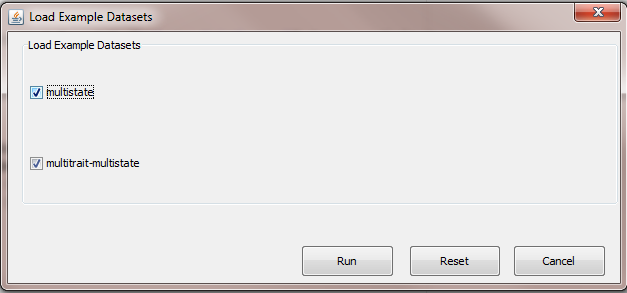
\includegraphics[scale=0.5]{loaddata.png}
  \label{fig:loaddata}
\end{figure}


Figure \ref{fig:lsttheory} shows a screenshot of the dialog for specifying the LST-R theory models. The dialog is a convenient graphical interface for the \texttt{lsttheory} function described previously. The graphical user interface provides easy access to almost all functionality described earlier in this vignette.


\begin{figure}
  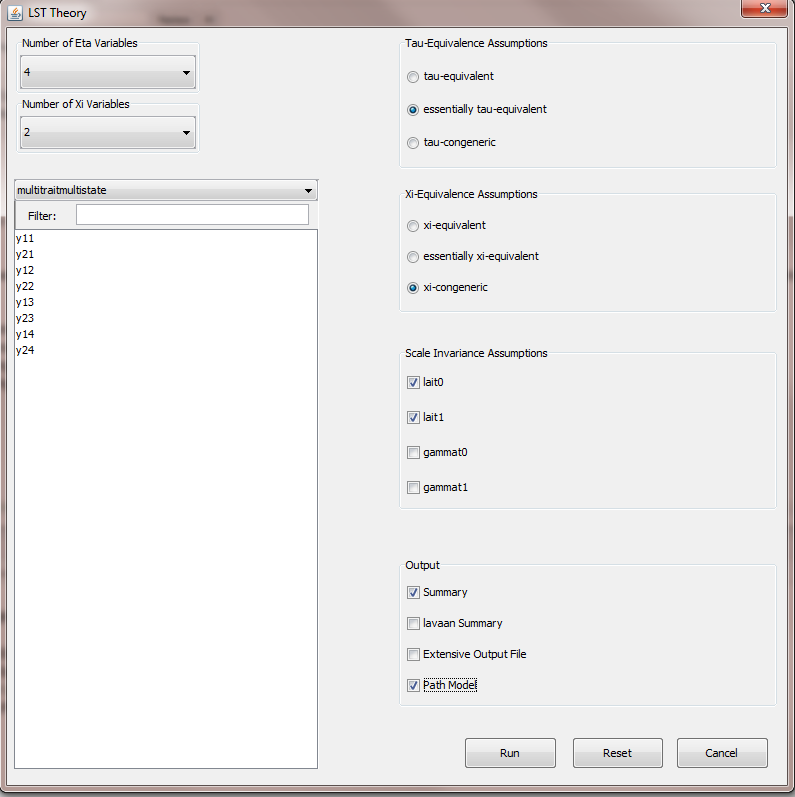
\includegraphics[scale=0.5]{lsttheory.png}
  \label{fig:lsttheory}
\end{figure}


\end{document}
